\documentclass{beamer}
\usetheme{Madrid}
\usepackage{graphicx}
\usepackage[T1]{fontenc}
% \usepackage[polish]{babel}
% \usepackage[polish]{datetime2}
\usepackage{graphicx}
\usepackage{caption}


\usepackage{tikz}
\def\checkmark{\tikz\fill[scale=0.4](0,.35) -- (.25,0) -- (1,.7) -- (.25,.15) -- cycle;} 


\title{Games classifier}

\author[Team name]{Team name\\[5mm]
{\small Members: Julia Cygan, Borys Adamiak, Patryk Flama}
\hspace{18mm} 
{\small Supervisor: Marek Adamczyk}}

\institute{UWr}
\date{\today}

\begin{document}

\begin{frame}
\titlepage
\end{frame}


\begin{frame}[t]{Goal and motivation}

{\bf Use case example:} \\
Imagine that you run a online game store where users can add their games to your library. Instead of manually checking if user tagged correctly the game, you can use our model to do that job for you. \\

\vspace{3mm}

{\bf Goal:} \\
We want to be able to automatically assign tags (or genres) to games, based on their (text) description.

\vspace{3mm}

Additionally, in aspect of ML project, we want to make a small comparison of different models and methods for solving such multilabel classification problem.
\end{frame}

\begin{frame}[t]{Info about the dataset}
Steam has its own official API, from which we downloaded games, their descriptions, tags and genres. That resulted in a bit over {\it 200'000} games. \\
\vspace{2mm}
To clean the data we:
\begin{itemize}
	\item Converted descriptions to alphanumeric lowercase
	\item Removed html tags
	\item Removed empty descriptions or tags
	\item (optional) Removed tags/genres that occured at most {\it n} times
\end{itemize}
After that we ended up with a dataset of size around {\it 50'000} games and {\it 400} unique tags or {\it 100} unique genres.

\end{frame}


\begin{frame}[t]{Data preprocessing}
\only<1-3>{
	To represent the output we decided to use multi label binary vector.
	
	\pause
	\vspace{3mm}

	For input preprocessing we tried:
	\begin{itemize}
		\item Bag of Words
		\item TF-IDF
		\item Hashing vectorizer
	\end{itemize}
	
	\pause
	\vspace{3mm}
	We decided to check if there are some patterns in the data that we can use to improve our model. \\
}

\pause
\only<4> {
	\vspace{-3mm}
	\begin{figure}[h]
		\caption{PCA analysis on Bag of Words}
		\centering
		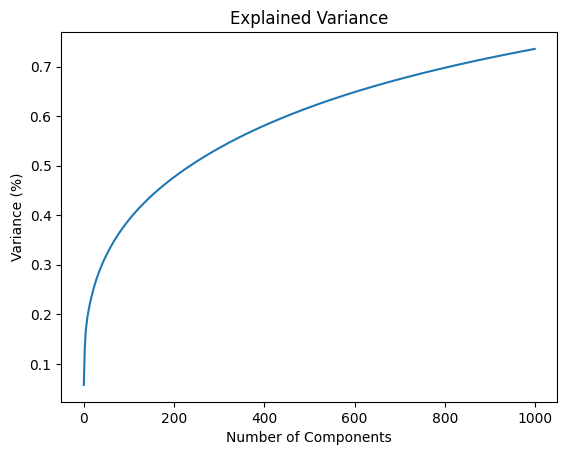
\includegraphics[width=0.73\linewidth]{images/pca_bow.png}
	\end{figure}
}

\pause
\only<5> {
	\vspace{-3mm}
	\begin{figure}[h]
		\caption{t-SNE 300 iterations + PCA to 50 on Bag of Words}
		\centering
		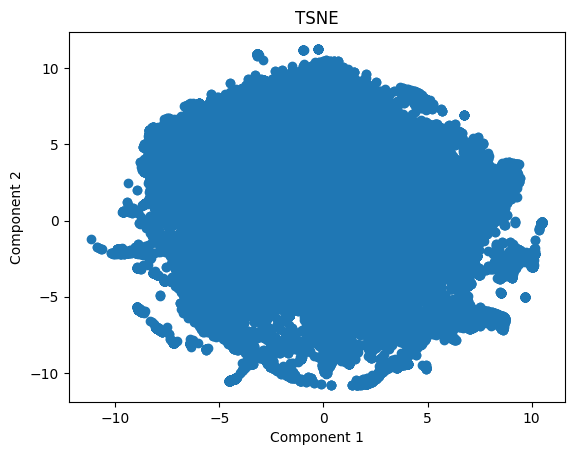
\includegraphics[width=0.73\linewidth]{images/tsne_300_bow.png}
	\end{figure}
}

\pause
\only<5>{
	Here is comparison of those methods on model using Logistic Regression and F1-score as evaluation metric:

	\begin{center}
		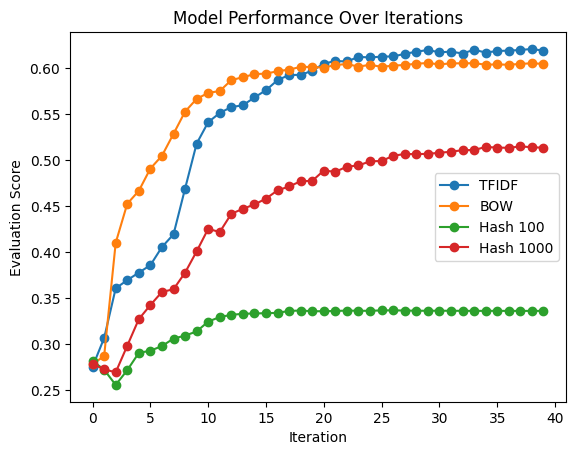
\includegraphics[width=0.73\linewidth]{images/LogisticRegression/f1score_compare_inprep.png}
	\end{center}
}

\end{frame}






\begin{frame}[t]{Models}

\begin{itemize}
    \item KNN \checkmark
    \item Logistic Regression \checkmark
    \item Decision Trees + Random Forest \checkmark
	\item Naive Bayes \checkmark
	\item Simple perceptron-based neural network \checkmark
	\item Support Vector Machine \checkmark
\end{itemize}
\end{frame}

\begin{frame}[t]{Evaluation}
\only<1-2>{
After analyzing the problem we came to conclusion that evaluaion methods are very interesing and important part of this project.

\pause

\begin{itemize}
	\item We dont want to falsely assign a tag to a game that should not have it
	\item Its more important to assing high percentage of tags to games, than to assign as many as possible
	\begin{itemize}
		\item Game should have 10 tags, but we only assign 8 (not bad)
		\item Game should have 1 tag, but we do not assign any (this is worse) 
	\end{itemize}
\end{itemize}
}

\pause

\begin{itemize}
\item Recall {\it TP/(TP+FN)} - we prefer to have more FN than to have an TP
 \checkmark
\item F1-score {\it (2 * precision * recall) / (precision + recall)} - nice name, but also it combines precision with recall thus both TP and FN are equally expensive \checkmark

\item Hammming loss
\item Intersection over union score
\item Exact match

\end{itemize}


\end{frame}


\begin{frame}[t]{Input data}
\only<1>{First we tried some unsupervised methods to check if we can find some patterns in the data}
	
\centering

\only<2-3>{
	PCA on Bag of Words representation of the data (to 10'000 words) \\
	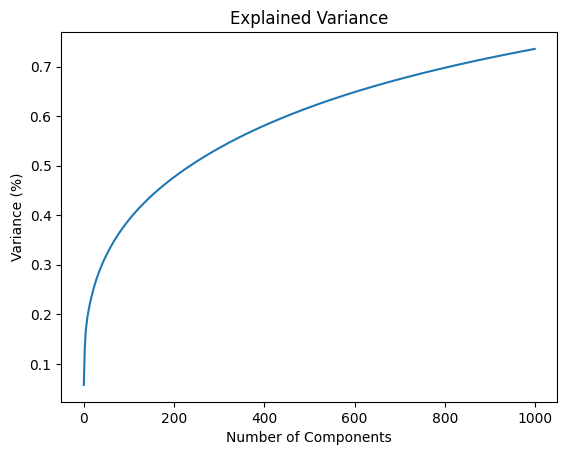
\includegraphics[width=0.6\textwidth,height=0.6\textheight,keepaspectratio]{images/pca_bow.png} % Replace with your image file
	
	\pause
	
	Nice, out of 10'000 dimensions we can create ~100 that 'explain' about half of the data.
}

\only<4-5>{
	t-SNE representation of same data \\
	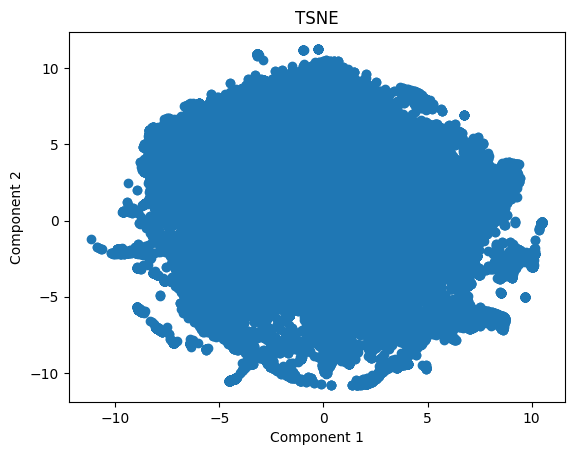
\includegraphics[width=0.6\textwidth,height=0.6\textheight,keepaspectratio]{images/tsne_300_bow.png} % Replace with your image file
	
	\pause
	
	And it does not look that helpful :<
}

\only<5-6>{
	But what about combining PCA with t-SNE?
}

\end{frame}

\end{document}